\IEEEPARstart{D}{iffusion}-based language models (DLLMs) have rapidly advanced from their thermodynamic origins to versatile generators across modalities. We trace this evolution in four stages.

\begin{figure*}[ht!]
    \centering
    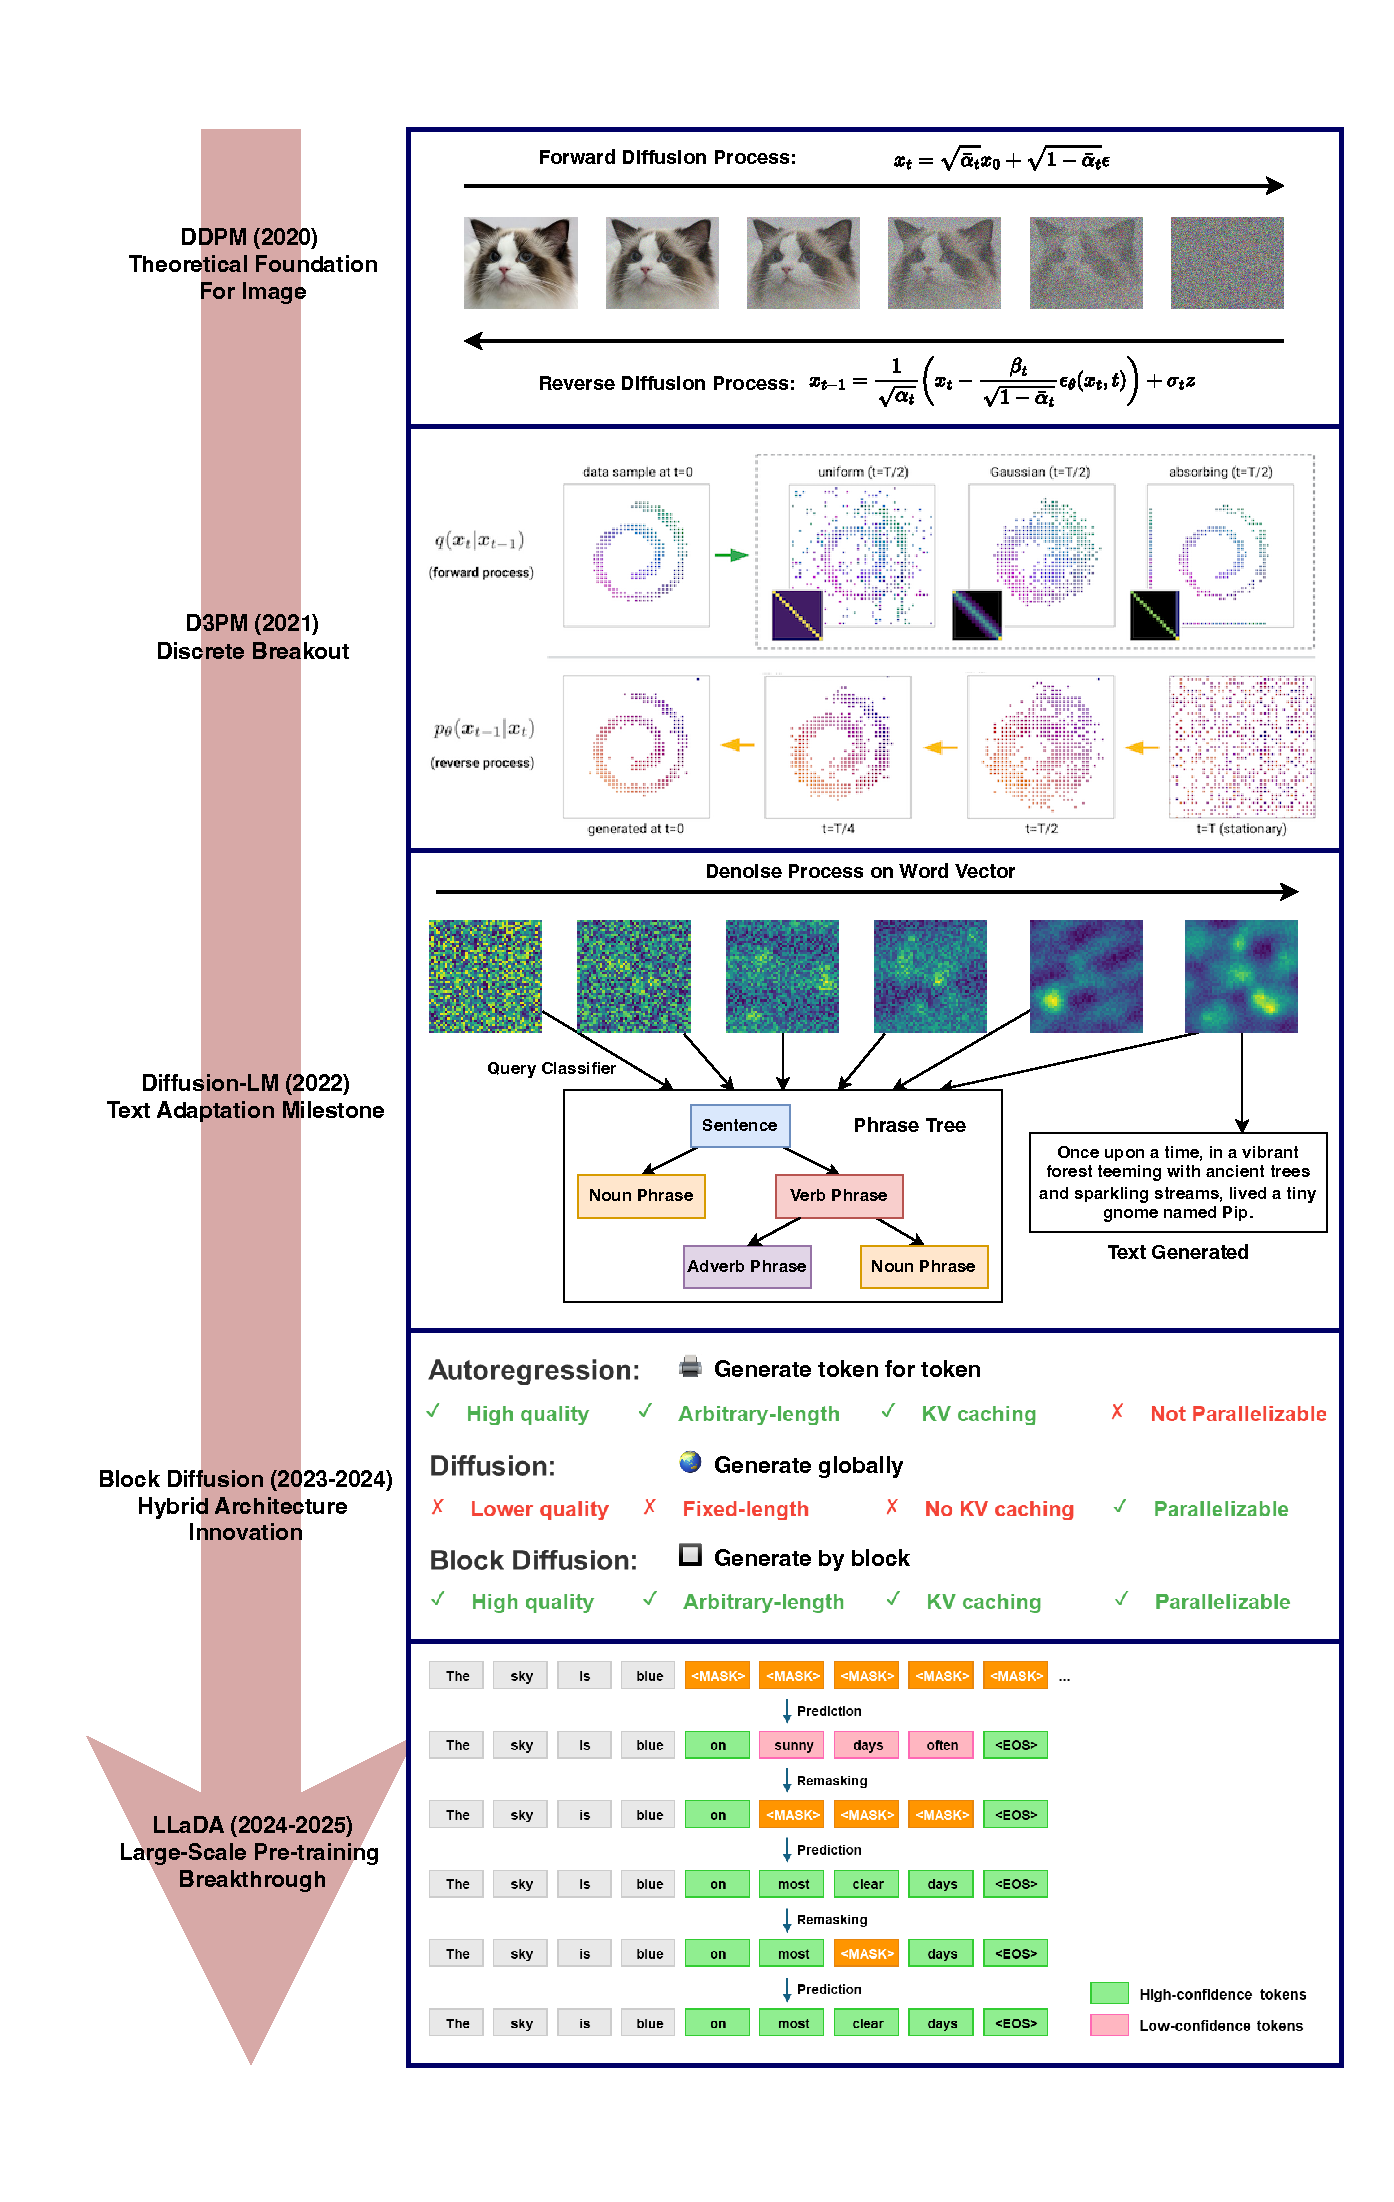
\includegraphics[width=0.7\textwidth]{figs/diffusion.pdf}
    \caption{\centering Evolution timeline of major diffusion model breakthroughs (2020-2025), demonstrating the progression from foundational frameworks to advanced hybrid architectures in generative AI.}
    \label{fig:diffusion}
\end{figure*}

\begin{figure*}[t]
    \centering
    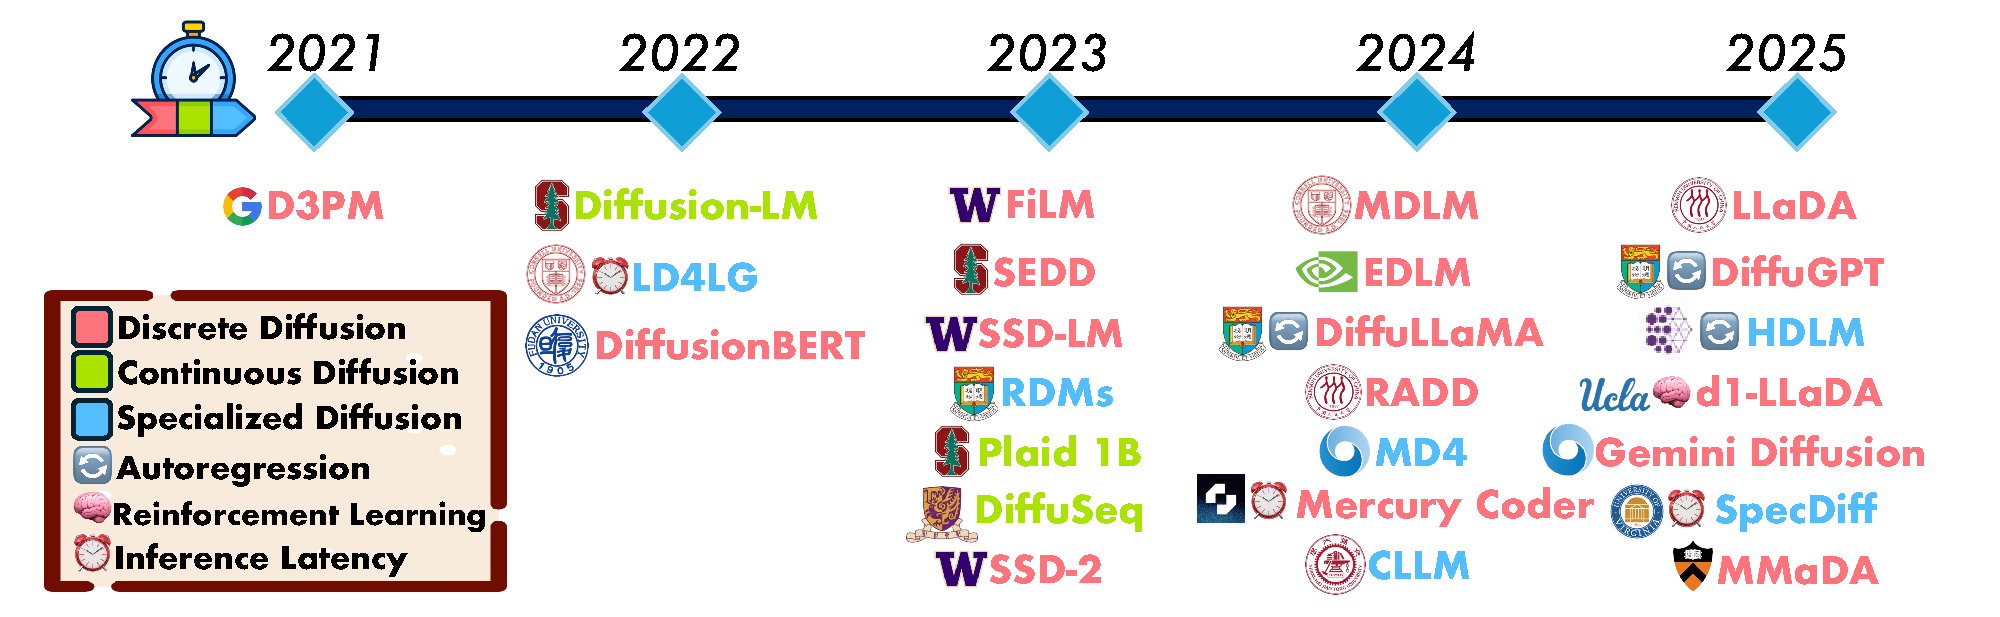
\includegraphics[width=0.95\textwidth]{figs/DLLMs_timeline.pdf}
    \caption{Evolution of key Diffusion Language Models (DLLMs) from 2021 to 2025, annotated by architectural innovations (e.g., discrete/continuous diffusion), integration with autoregression or reinforcement learning, and inference efficiency breakthroughs.}
    \label{fig:timeline}
\end{figure*}

\subsection{Early Foundations (2015–2020)}
The original \textbf{Denoising Diffusion Probabilistic Models (DDPM)} introduced a Markovian forward and reverse noising chain on continuous data, establishing the core variational framework for diffusion-based generation \cite{ho_denoising_2020}. Building on this, \textbf{Denoising Diffusion Implicit Models (DDIM)} generalized DDPM sampling to a non-Markovian family of deterministic or accelerated trajectories, while preserving the same training objective \cite{song_denoising_2020}. To handle discrete data, Hoogeboom \emph{et al.} proposed \textbf{Structured Denoising Diffusion Models in Discrete State-Spaces (D3PM)}, which uses absorbing-state kernels without explicit timestep embeddings \cite{hoogeboom_structured_2021}.

\subsection{First Text-Specific Adaptations (2021–2022)}
Zou \emph{et al.} provided the first systematic survey of diffusion for non-autoregressive text generation, defining both discrete (mask-based) and continuous (Gaussian embedding) formulations and demonstrating their parallelism and controllability advantages over prior NAR methods \cite{zou_survey_2023}. Hoogeboom’s D3PM work showed that absorbing-state discrete diffusion can produce coherent categorical samples without timestep inputs \cite{hoogeboom_structured_2021}. Concurrently, \textbf{Diffusion-LM} embedded Gaussian noise into token representations and outperformed earlier controllable generation models on sentiment and syntax tasks \cite{li_diffusion-lm_2022}. Subsequent innovations included Dieleman \emph{et al.}’s continuous diffusion on one-hot vectors with specialized rounding \cite{dieleman_continuous_2022}, Strudel \emph{et al.}’s self-conditioned embedding diffusion \cite{strudel_selfconditioned_2021}, and transformer-based ODE–diffusion hybrids such as Difformer \cite{gong_difformer_2022} and Composable Text Controls \cite{liu_composable_2022}. Han \emph{et al.} introduced SSD-LM, a semi-autoregressive simplex diffusion reducing denoising steps by half while preserving translation quality \cite{han_ssdlm_2022}, and Yuan \emph{et al.}’s SeqDiffuSeq demonstrated parallel seq2seq decoding in under 30 steps \cite{yuan_seqdiffuseq_2021}.

\subsection{Hybridization and Architectural Innovations (2023–2024)}
The hybrid paradigm emerged with \textbf{}{Block Diffusion}, which interleaves autoregressive first-token sampling with blockwise diffusion to balance sequential fidelity and parallel speed \cite{arriola_block_2025}. \textbf{Latent Diffusion for Language Generation} projects token embeddings into a compact latent space for diffusion, then reconstructs via an AR decoder, achieving significant speedups without quality loss \cite{lovelace_latent_2023}. Energy-based approaches like \textbf{DiffPO} use a pretrained AR model as an energy function to reweight diffusion samples, reducing decoding error with fewer steps \cite{xu_energy-based_2025}. \textbf{Speculative Diffusion Decoding} treats a fast DLLM as a draft generator and an AR model as verifier, enabling near-AR quality with reduced sequential passes \cite{christopher_speculative_2025}. Task-specific optimizations, such as SSD-2’s inference-time fusion of small and large diffusion LMs, further improved throughput and privacy by splitting computation \cite{han_david_2024}.

\subsection{Recent Advances and Generalization (2024–2025)}
Recent work has extended DLLMs to multimodal and instruction-tuned scenarios. \textbf{HybridVLA} unifies vision, language, and action diffusion in a single model for embodied agent tasks \cite{liu_hybridvla_2025}. Studies on instruction fine-tuning, such as those by Zhou \emph{et al.}, demonstrate that diffusion LLMs can generalize zero-shot to unseen languages and tasks after English-only SFT \cite{nie_large_2025}. Comprehensive surveys highlight classification and benchmarking of DLLM capabilities across domains, marking the maturation of diffusion methods in NLP and beyond.

Together, these stages—from continuous DDPM through discrete D3PM, early NAR text diffusion, hybrid block and latent architectures, to multimodal and instruction-tuned generalists—chart the swift evolution of DLLMs into powerful, flexible generators.  

% \bibliographystyle{ieeetr}
% \bibliography{DLLM}
